
Imagine the following scenario (inspired by the YouTube channel:[]):
Today we are going to draw a smiling ice-cream cone. Okay, we are going to first draw a curve as the top of a big scoop of ice-cream. Next, we will draw a sequence of connected U's to represent the bottom of the overflowing ice-cream. Lastly, we will draw a large upside-down triangle as the cone of our ice-cream.

We want to realize this kind of interactions with a robot, as a companion, so we need to collect a dataset that can help us to get closer to this goal. In order to study this problem, we want to collect human sketches, so the first thing we did was designing an web interface.  
The leading questions of the data collection process. Our goal is to collect a dataset so that we can learn a model that can interactively draw sketches with users. Therefore, we want to collect the drawing for a single step and a person's description of the drawing. Our design of the interface centers around some key questions: 
\begin{enumerate}
    \item \label{data_design_3} Ensure that the drawing responds to the prompt. The underlying assumption here is that the prompt itself will give us some signals in terms of where the objects in the images might be.  
    \item \label{data_design_1} From the design side, enforce annotators to breaking the sketch generation process into steps. The worst scenarios is for the annotators to   
    \item \label{data_design_2} How do we make sure that annotators are breaking the sketches they provide into reasonable steps? What we mean by reasonable here is the fact that there should be a good correspondence between some parts of the sketch and the language that is used to describe it. Although in our daily interactions, we might say something like ``we now draw this'' or ``we can do this'', but from a model learning perspective, or more so as a first step, we want there to be little ambiguity in our language and disallowing words like ``this''.     
    % {\color{red} \faIcon{question}} How to make sure that users can do not go outside the step? How to make sure that users do not miss a step? How to make sure that users do not cram two steps together? How to make sure that they remember to annotate for a step and also give the accurate descriptions? 
\end{enumerate}



% \setlist[enumerate,1]{leftmargin=12mm}
% \begin{enumerate}[itemsep=6pt,topsep=6pt]
%   \usageitem{\centering \faBook} \label{test_1} \textbf{Dictionary} is ...
%   \usageitem{\centering \large \faIcon{phone-square-alt}} \textbf{Mobile phones} are cool ...
% \end{enumerate}
% Reflects main requirement \ref{test_1}{\faBook}

Our interface has experienced 2 main versions, and the major difference between the two is that the first one asks users to draw the sketches and annotate each step in their drawings while the second version asks the users to annotate existing sketches. The turning point happens after a pilot deployment of the first version, during which we identified several problems: (1) users take too long to complete one task, and it is outside our budge to collect an ample dataset; (2) users cannot separate the entire sketch into steps consistently, and the annotations either describe more or less than what was done in a single step. In order to shorten the task time and alleviate the burden to think about how to draw certain objects, our second version uses sketches from the Quick,Draw! dataset collected by Google and asks users to provide textual annotations for each part in the sketches. The following sections will walk through each version and discuss the data collected using each version. The following sections will walk through each version and discuss how the design reflects or answers the above N criteria and what in reality happened that caused us to change the design.  

Later, we discovered that by simply using existing sketches without asking for users to draw for the prompt would significantly reduce the data collection time, and it would also allow us to put aside DQ \ref{data_design_1}. In general, if you think about it, classic collection tasks such as assigning label to images/texts or drawing segmentation box, the goal of the task is very clear, and it is easy to determine the quality of the work when you glance at it, or easy to verify. At the beginning, we found it very difficult to describe what should be drawn and what should not be drawn, or what can be written and what cannot be written. 

The general trend of the data collection process is that we try to simplify the data collection interface and reduce the number of criteria that we need to satisfy, since each introduces a factor of uncertainty. 

Since the beginning of data collection, an important question we try to answer is how do we define a semantic unit in the sketch?  
The end goal is to achieve the kind of interaction shown in the YouTube video \textit{How To Draw A Cute Ice Cream Cone}, and in it, the instructor oftens uses sentences in the form of ``Let's draw a \texttt{X} for \texttt{Y}'', where \texttt{X} describes the geometric features of the object \texttt{Y}. For example, ``Let's draw \textit{small connected U shapes} for the \textit{bottom of the ice-cream cone}.'' Therefore, at first, we thought of decomposing the drawing process into a sequence of common geometric shapes, and the objects that they represent become the basic semantic units.      
At each step, the annotator is first asked to 
Version 0 was never deployed. I think at this stage of the data collection, we are trying to decide whether there should be a fixed set of primitive that the users could choose from, so learning the model becomes learning to parameterize, for example, the dimensions of the set of primitives. 

Functionality:
\begin{itemize}
    \item Draw the figure and the page will record the sequence 
    \item User can replay its drawing sequence. The original idea was that users will first create the drawing, and then they can replay the sequence as they annotate for each step. 
\end{itemize}

The very first test version:
In terms of the main task, I created a test version to confirm that the idea of the drawing board is sensible.

Press \textit{Record}, Draw on the board, Press \textit{Stop} when done with drawing, \textit{Submit} the drawing if one is satisfied with the quality, \textit{Play} to revisit the drawing, \textit{Cancel} to start over. 

What was the original motivation behind this functionality was that it will aid the annotators to review the drawing process and divide it into better steps. Responding to DQ \ref{data_design_1}. 
However, in this very crude version, we did not really incorporate features for either 
Responding to DQ \ref{data_design_2}, 

We begin with a very crude version, and then we decide to add features that can allow us to realize the DQ \ref{data_design_1} and \ref{data_design_2}.

The actual Version 0 has the following flow:
There is a practice board, you can try to practice drawing so that the actual drawing submit has good quality and respond to the prompt (reflecting DQ \ref{data_design_3}). Then hit \textit{Ready to Record}, again baking the sequence into the design of the website will help us to enforce collecting a dataset of steps. Another purpose is to help the annotators decide beforehand what are the necessary primitives used in the process. Why was I so fixated on the primitives, because the abstractness of the icons is what interested me the most. The entire research journey was very explorative, it sorted of started with a sense of \textit{oh, this question or aspect of how humans do things is interesting, I wish robot can do the same}. And what is that thing that I thought was interesting, it was how Rain and I were able to draw the icons and the interactions. 
The first thing you will do is select a primitive from a list, and then you will draw the step that contains the primitives. Hit \textit{Next} to move on to drawing the next primitive. There are will be a little tag at the bottom showing what is the primitive that corresponds to the step that is drawn on the board. Repeat until finished and hit \textit{Done}. At the end, again, \textit{Play}, \textit{Submit}, or \textit{Cancel} to start over. 

{\color{red} \faIcon{question}} Should we use primitive shapes for users to choose from? 
The reason for considering this aspect is whether during generation we want to learn to change parameters of a fix set of shapes or generate un-constrained strokes. For the first option, we want users to compose a drawing with primitive shapes, much like using   
In order to learn a more general model, we decided that we want to collect strokes instead of fixed primitive shapes, so we moved onto creating a table that accompanies the drawing board, where the user can choose to annotate each step they draw. 

In Figure \ref{v0.design}. 

\begin{figure*}[ht!]
\begin{subfigure}{\textwidth}
  \centering
  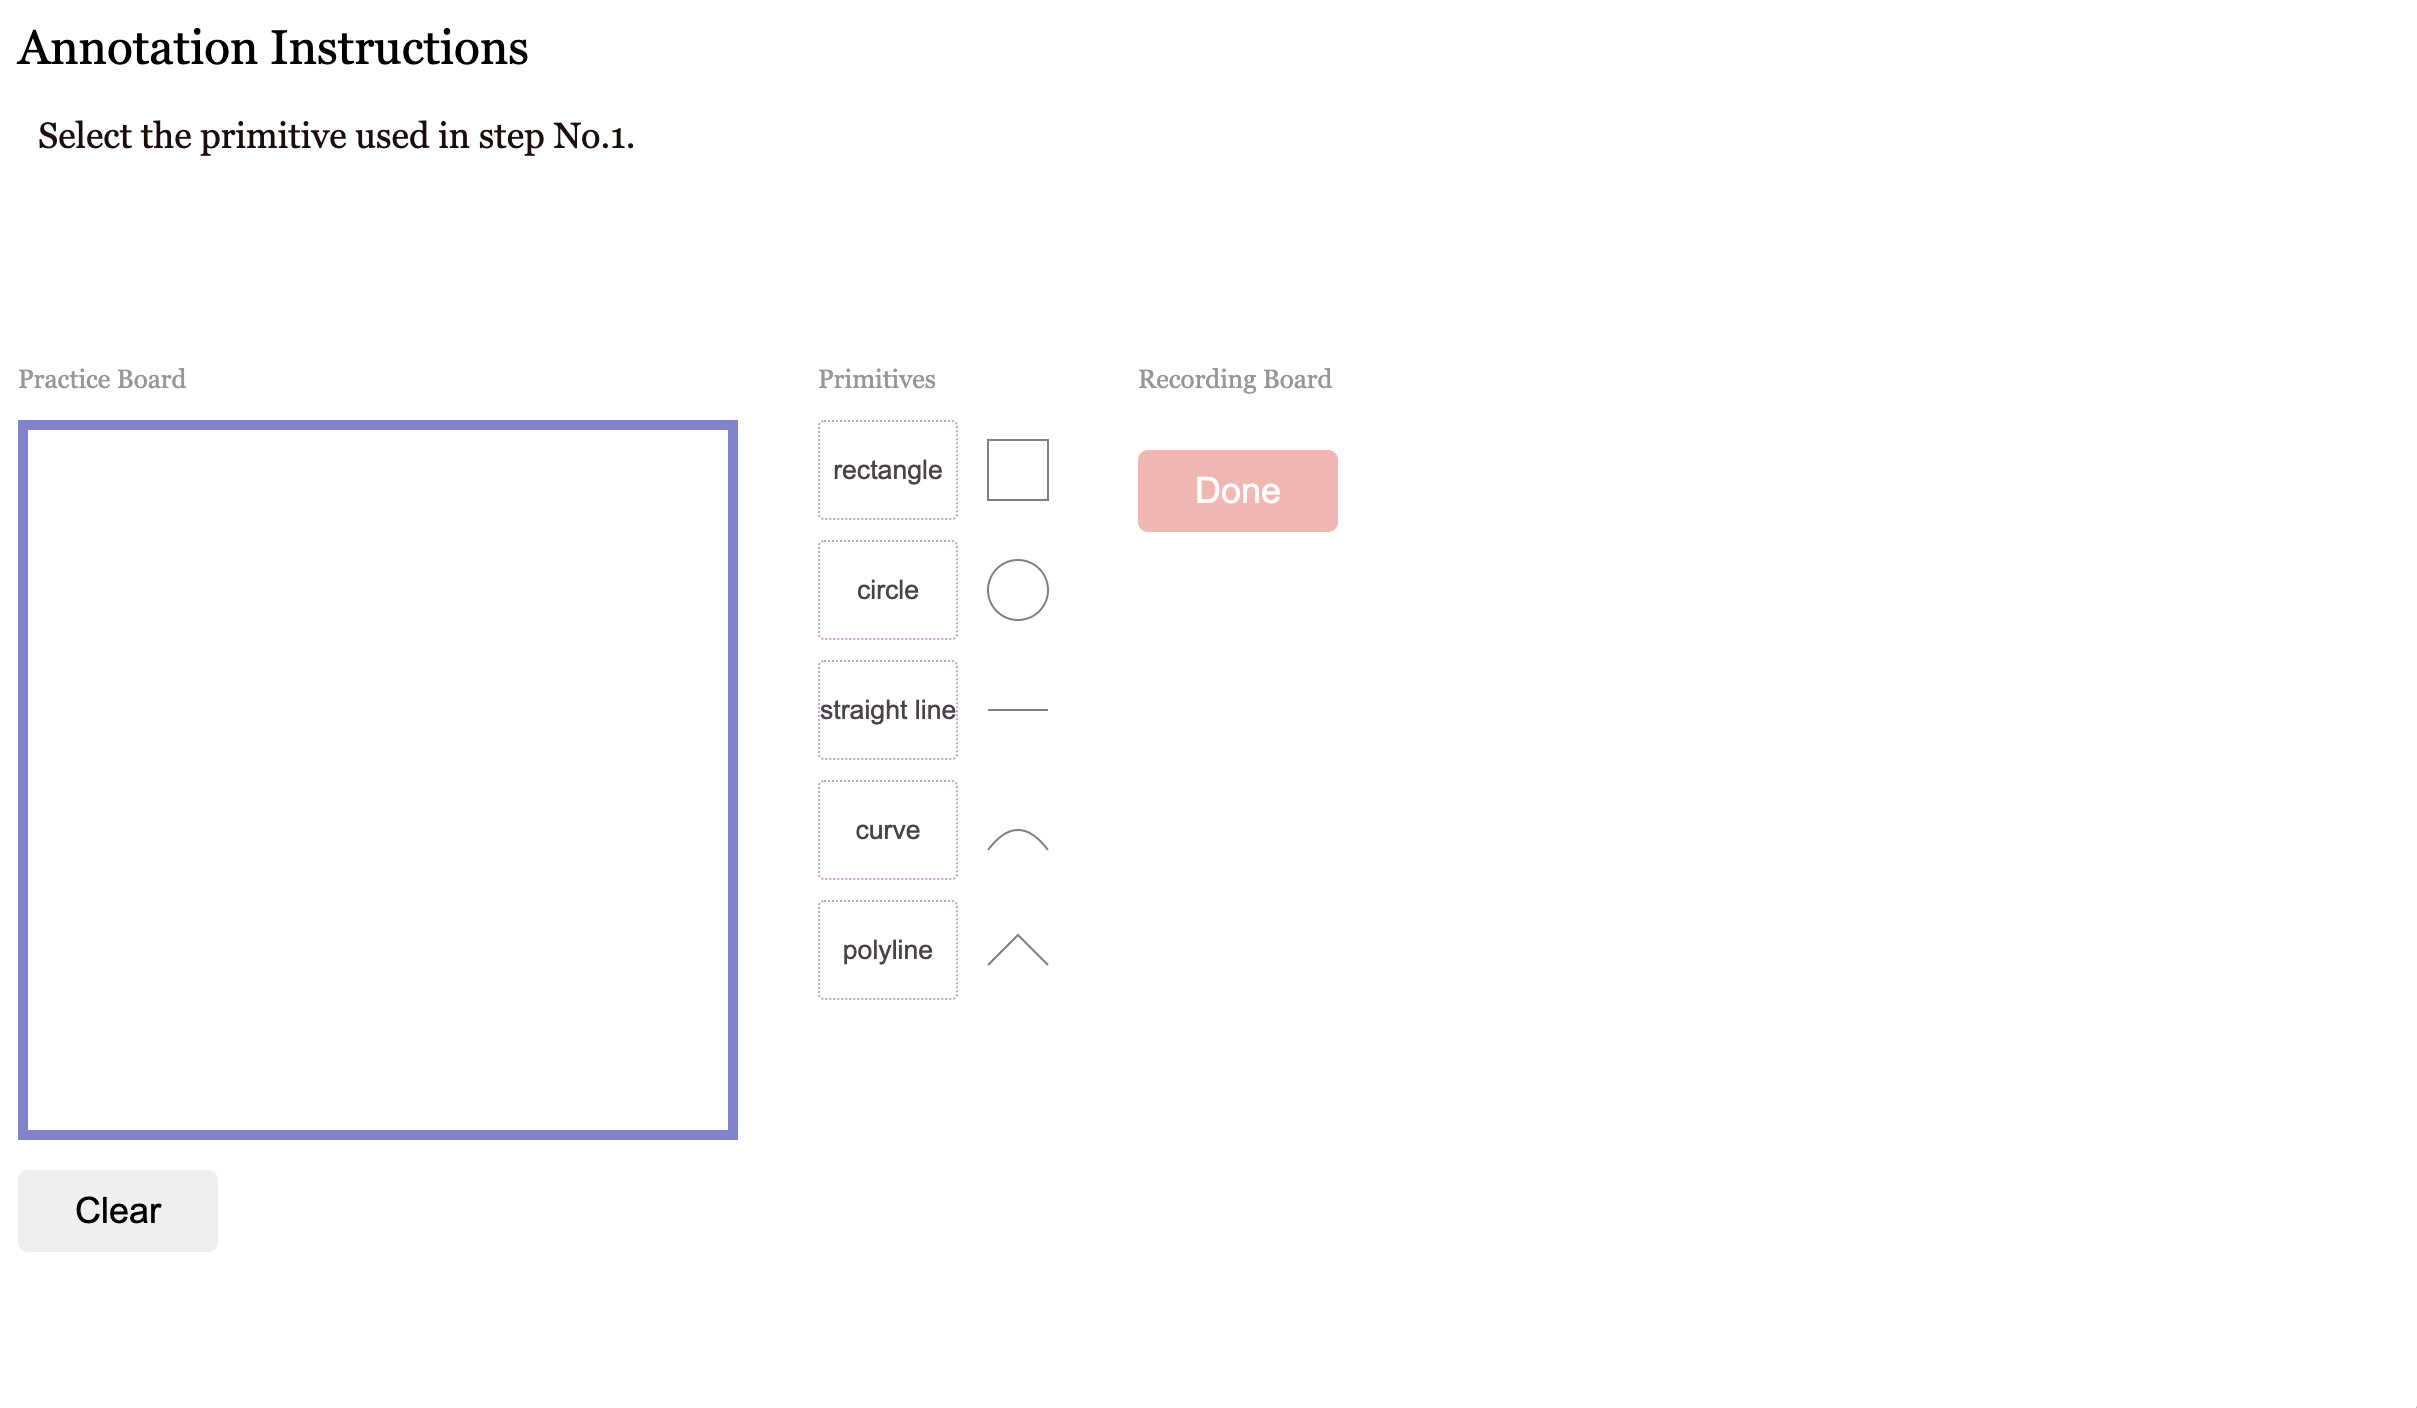
\includegraphics[width=.8\linewidth]{data_collection/version_0_select_primitive.png}
  \caption{Design of main task for third pilot.}
  \label{v0.1}
\end{subfigure}
\newline
\begin{subfigure}{\textwidth}
  \centering
  % include third image
  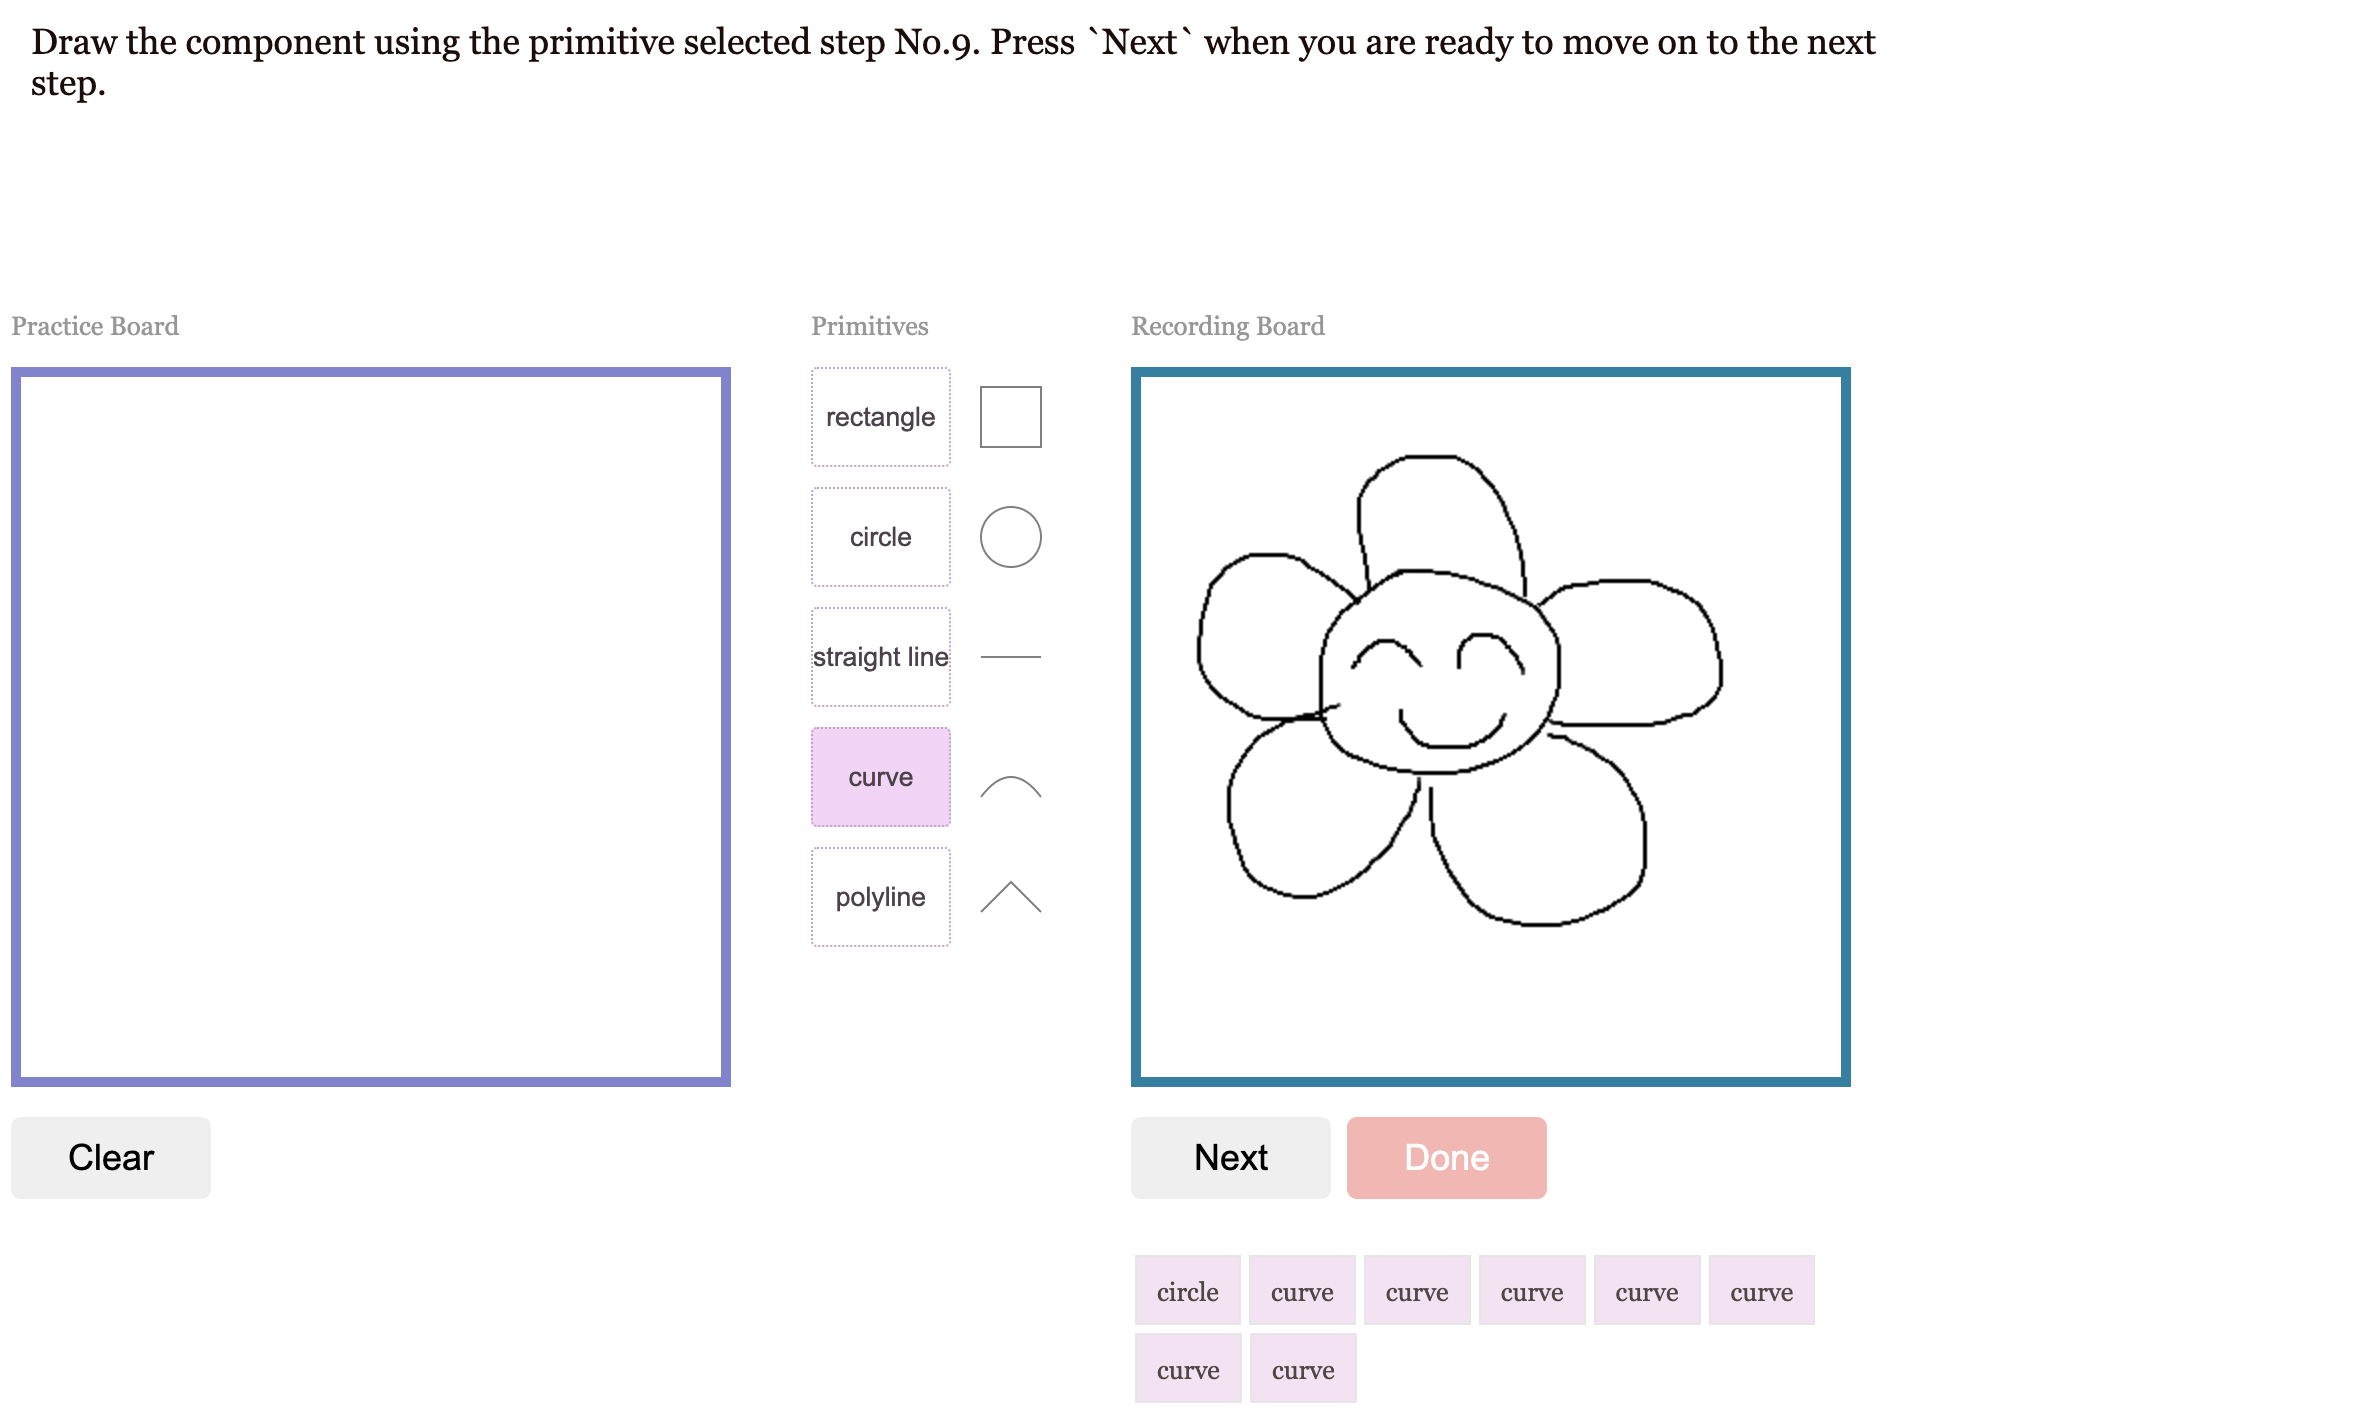
\includegraphics[width=.8\linewidth]{data_collection/version_0_smiley_flower_with_primitive.png}  
  \caption{Design of main task for final task.}
  \label{v0.2}
\end{subfigure}
\caption{Progress of the design two for the main task in version two.}
\label{v0.design}
\end{figure*}